\newpage
\subsection{UC4 - Modifica visualizzazione}
\label{sub:uc4}

%TODO: Add correct image
\begin{figure}[h]
    \centering
    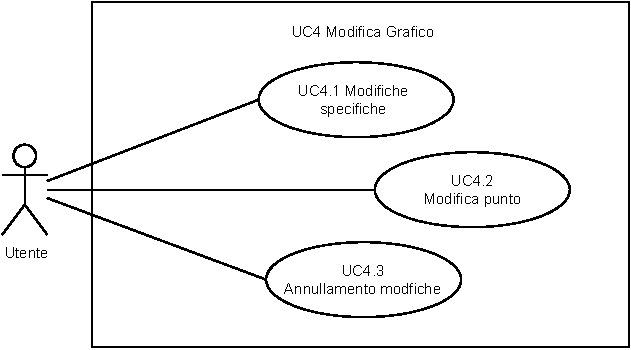
\includegraphics[width=0.8\textwidth]{componenti/casi-duso/diagrammi/UC4.pdf}
    \caption{Diagramma rappresentante UC4}
    \label{fig:UC4}
\end{figure}


\begin{itemize}
    \item \textbf{Descrizione}: L’utente modifica il grafico attuale del quale viene fornita la visualizzazione aggiornata.
	
    \item \textbf{Attore primario}: Utente.
    
    \item \textbf{Precondizione}:   È stato costruito correttamente un grafico (\hyperref[sub:uc2]{UC2})

    \item \textbf{Postcondizione}:  Viene visualizzato il grafico modificato con i nuovi parametri.

	\item \textbf{Scenario principale}:
		\begin{enumerate}
            \item L'utente modifica i parametri di visualizzazione, interagendo con gli strumenti resi disponibili dal grafico che sta visualizzando,
                    dal menu di modifica.
            \item La visualizzazione del grafico viene aggiornata in accordo con i parametri modificati.
        \end{enumerate}

    \item \textbf{Scenario alternativo}:
        \begin{enumerate}
            \item L'utente seleziona la voce "Annulla" dal menù di modifica.
            \item Le modifiche vengono scartate e viene ripristinata la visualizzazione del grafico precedente.  (\hyperref[ssub:uc4.8]{UC4.8})
        \end{enumerate}
    
\end{itemize}

\newpage
\subsubsection{UC4.1 Modifica grafico}
\label{ssub:uc4.1}

\begin{itemize}
    \item \textbf{Descrizione}: L’utente effettua modifica specifiche al tipo di grafico precedentemente costruito e visualizzato, 
                                su parametri quindi validi solo per tale visualizzazione, e ne vede le modifiche.
	
    \item \textbf{Attore primario}: Utente.
    
    \item \textbf{Precondizione}:   È stato costruito correttamente un grafico. (\hyperref[sub:uc2]{UC2})

    \item \textbf{Postcondizione}:  Viene aggiornato il grafico costruito e visualizzato con i nuovi parametri.

    \item \textbf{Generalizzazioni}:
        \begin{itemize}
            \item Modifica Scatterplot Matrix (\hyperref[ssub:uc4.2]{UC4.2})
            \item Modifica a grafico con Matrice delle Distanze (\hyperref[ssub:uc4.3]{UC4.3})
            \begin{itemize}
                \item Modifica Force Field (\hyperref[ssub:uc4.4]{UC4.4})
                \item Modifica Distance Map (\hyperref[ssub:uc4.5]{UC4.5})
             \end{itemize}
            \item Modifica Heat Map (\hyperref[ssub:uc4.6]{UC4.6})
            \item Modifica Proiezione Lineare Multi Asse (\hyperref[ssub:uc4.7]{UC4.7})
        \end{itemize}
\end{itemize}

\subsubsection{UC4.2 Modifica Scatterplot Matrix}
\label{ssub:uc4.2}

\begin{figure}[h]
    \centering
    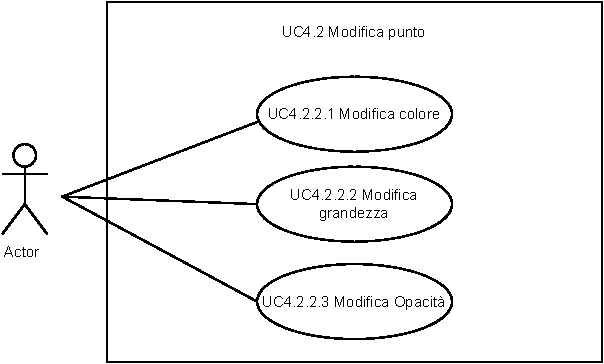
\includegraphics[width=0.6\textwidth]{componenti/casi-duso/diagrammi/UC4_2.pdf}
    \caption{Diagramma rappresentante UC4.2}
    \label{fig:UC4.2}
\end{figure}


\begin{itemize}
    \item \textbf{Descrizione}: L’utente modifica la visualizzazione dello Scatterplot Matrix
                                costruito dal dataset corrente.
	
    \item \textbf{Attore primario}: Utente.
    
    \item \textbf{Precondizione}:   La visualizzazione costruita dal dataset corrente è uno Scatterplot Matrix.

    \item \textbf{Postcondizione}:  Viene aggiornato il grafico costruito e visualizzato con i nuovi parametri.

	\item \textbf{Scenario principale}:
		\begin{enumerate}
            \item L'utente apporta le modifiche desiderate tra quelle offerte dallo Scatterplot Matrix.
        \end{enumerate}
\end{itemize}


\paragraph{UC4.2.1 Modifica dimensioni della matrice}
\label{par:uc4.2.1}
\begin{itemize}
    \item \textbf{Descrizione}:     L’utente dispone di dati con metadati assegnati e può 
                                    scegliere fino a 5 dimensioni che possono essere visualizzate nello Scatter Plot 
                                    Matrix.
	
    \item \textbf{Attore primario}: Utente.
    
    \item \textbf{Precondizione}:   La visualizzazione costruita dal dataset corrente è uno Scatterplot Matrix.
    \item \textbf{Postcondizione}:  Vengono modificate le dimensioni visualizzate nei plot dello Scatter Plot Matrix.

	\item \textbf{Scenario principale}:
        \begin{enumerate}
            \item   L'utente seleziona l'opzione di selezione delle dimensioni.
            \item   L'utente seleziona fino a cinque dimensioni. 
           
            \item   Ad ogni selezione l'utente
                    sceglie una delle dimensioni attuali del grafico e la scarta.
           
            \item   La visualizzazione sostituisce le dimensioni scartate con le nuove selezionate.
        \end{enumerate}
\end{itemize}

\paragraph{UC4.2.2 Modifica dimensione rappresentata mediante tinta}
\label{par:uc4.2.2}
\begin{itemize}
    
    \item \textbf{Descrizione}:     L'utente assegna ad una dimensione un insieme di tinte per poterla rappresentare 
                                    graficamente;
    
    \item \textbf{Attore primario}: Utente;
    \item \textbf{Precondizione}:   La visualizzazione correntemente costruita dal dataset è uno Scatter Plot Matrix;
    \item \textbf{Postcondizione}:  Viene aggiunta una dimensione rappresentata mediante tinta;
    \item \textbf{Scenario principale}:
    \begin{enumerate}
        
        \item   Interagendo con l'apposito pulsante, l'utente seleziona la dimensione che desidera rappresentare 
                mediante tinta, sostituendo così quella precedente;

        \item   L'utente seleziona tra gli intervalli di tinte suggeriti quello con cui i diversi elementi della 
                dimensione scelta saranno visualizzati;
        
        \item   La visualizzazione viene aggiornata in accordo con le modifiche effettuate.
    \end{enumerate}
\end{itemize}

\paragraph{UC4.2.3 Modifica dimensione rappresentata mediante brillanza}
\label{par:uc4.2.3}
\begin{itemize}

    \item \textbf{Descrizione}:     L'utente assegna ad una dimensione la rappresentazione mediante brillanza;
    \item \textbf{Attore primario}: Utente;
    \item \textbf{Precondizione}:   La visualizzazione correntemente costruita dal dataset è uno Scatter Plot Matrix;
    \item \textbf{Postcondizione}:  Viene modificata la dimensione rappresentata mediante brillanza;
    \item \textbf{Scenario principale}:
    \begin{enumerate}
        \item   Interagendo con l'apposito pulsante, l'utente seleziona la dimensione che desidera rappresentare 
                mediante brillanza, sostituendo così quella precedente;

        \item   La visualizzazione viene aggiornata in accordo con la modifica effettuata.
    \end{enumerate}
\end{itemize}

\paragraph{UC4.2.4 Selezione punto}
\label{par:uc4.2.4}
\begin{itemize}
    \item \textbf{Descrizione}: L'utente seleziona un punto in uno Scatterplot della matrice per vedere come 
                                esso viene rappresentato negli altri grafici a dispersione della visualizzazione corrente.
	
    \item \textbf{Attore primario}: Utente.
    
    \item \textbf{Precondizione}:   La visualizzazione costruita dal dataset corrente è uno Scatterplot Matrix.
    \item \textbf{Postcondizione}:  Le proiezioni del punto selezionato, se appartiene al dataset importato, 
                                    vengono evidenziate in tutti i grafici della visualizzazione.

	\item \textbf{Scenario principale}:
        \begin{enumerate}
            \item L'utente seleziona un punto contente dati di uno Scatterplot della matrice.
            \item La proiezione del punto viene evidenziata in tutti gli Scatterplot della visualizzazione.
        \end{enumerate}

    \item \textbf{Scenario alternativo}:
        \begin{enumerate}
            \item L'utente seleziona un punto che non rappresenta nessun dato del dataset.
            \item Non viene evidenziato alcun punto della matrice.
        \end{enumerate}

\end{itemize}


\paragraph{UC4.2.5 Selezione insieme di punti}
\label{par:uc4.2.5}
\begin{itemize}
    \item \textbf{Descrizione}: L'utente seleziona un insieme di punti in uno Scatterplot della matrice per vedere come 
                                essi vengono rappresentati negli altri Scatterplot della matrice.
	
    \item \textbf{Attore primario}: Utente.
    
    \item \textbf{Precondizione}:   La visualizzazione costruita dal dataset corrente è uno Scatterplot Matrix.
    \item \textbf{Postcondizione}:  Le proiezioni degli insiemi di punti selezionati, se appartenente al dataset importato, 
                                    vengono evidenziate in tutti i grafici della visualizzazione.

	\item \textbf{Scenario principale}:
        \begin{enumerate}
            \item L'utente seleziona un insieme di punti di uno Scatterplot della matrice.
            \item Le proiezioni dei punti contenenti dati vengono evidenziati in tutti gli Scatterplot della visualizzazione.
        \end{enumerate}

    \item \textbf{Scenario alternativo}:
        \begin{enumerate}
            \item L'utente seleziona un insieme di punti vuoto.
            \item Non viene evidenziato alcun punto della matrice.
        \end{enumerate}

\end{itemize}

\newpage
\subsubsection{UC4.3 Modifica a grafico con matrice delle distanze}
\label{ssub:uc4.3}

% TODO: Insert UC4.3 image
\begin{figure}[h]
    \centering
    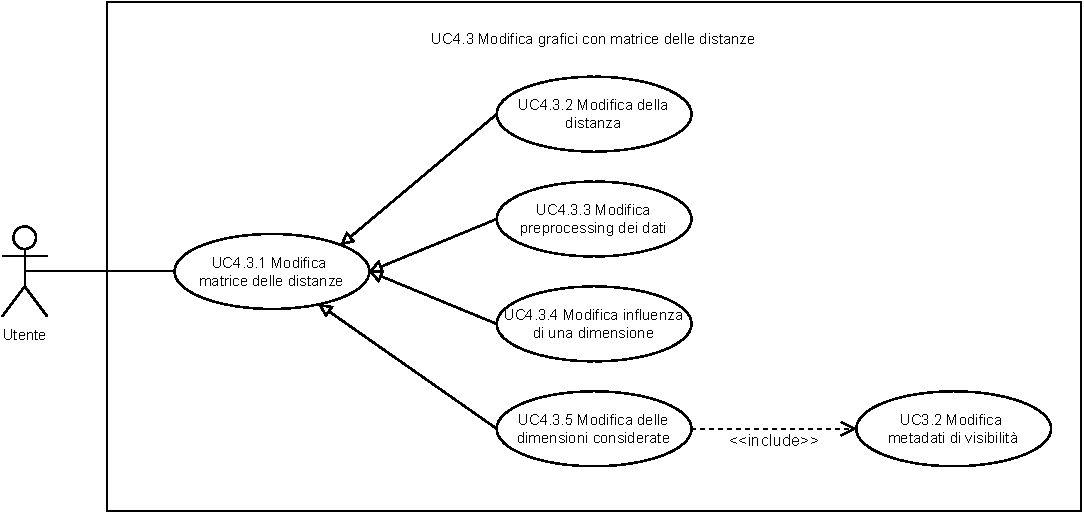
\includegraphics[width=0.8  \textwidth]{componenti/casi-duso/diagrammi/UC4_3.pdf}
    \caption{Diagramma rappresentante UC4.3}
    \label{fig:UC4.3}
\end{figure}

\begin{itemize}
    \item \textbf{Descrizione}: L’utente vuole modificare la visualizzazione di un grafico che sfrutta la matrice delle distanze
                                nella sua costruzione, quindi un Force Field o una Distance Map.
    \item \textbf{Attore primario}: Utente.
    \item \textbf{Precondizione}: La visualizzazione costruita dal dataset corrente è una Force Field o una Distance Map.
    \item \textbf{Postcondizione}: Viene aggiornato il grafico costruito e visualizzato con i nuovi parametri.
    \item \textbf{Scenario principale}:
    \begin{enumerate}
        \item   L’utente apporta le modifiche desiderate tra quelle offerte dal grafico con matrice
                delle distanze e quelle specifiche al tipo di grafico che la visualizzazione attuale rappresenta.
    \end{enumerate}
    \item \textbf{Generalizzazioni}:
    \begin{itemize}
        \item Modifica Force Field. (\hyperref[ssub:uc4.4]{UC4.4})
        \item Modifica Distance Map. (\hyperref[ssub:uc4.5]{UC4.5}) 
    \end{itemize}
\end{itemize}

\paragraph{UC4.3.1 Modifica della distanza}
\label{par:uc4.3.1}
\begin{itemize}
    \item \textbf{Descrizione}: L’utente decide di cambiare l’algoritmo usato per il calcolo delle distanze.

    \item \textbf{Attore primario}: Utente.
    
    \item \textbf{Precondizione}:   L'utente ha selezionato la voce di \emph{"Modifica della distanza"} da (\hyperref[ssub:uc4.3]{UC4.3}).
    \item \textbf{Postcondizione}:  La visualizzazione corrente viene aggiornata in rapporto ai nuovi valori della matrice.

	\item \textbf{Scenario principale}:
        \begin{enumerate}
            \item L'utente seleziona uno degli algoritmi presentati dalla modifica della distanza.
            \item La visualizzazione modifica la distanza tra i punti secondo l'algoritmo scelto.
        \end{enumerate}
\end{itemize}

\paragraph{UC4.3.2 Modifica preprocessing dei dati}
\label{par:uc4.3.2}
\begin{itemize}
    \item \textbf{Descrizione}: L’utente sceglie se normalizzare o standardizzare i dati.

    \item \textbf{Attore primario}: Utente.
    \item \textbf{Precondizione}: L'utente ha selezionato la voce di \emph{"Modifica preprocessing dei dati"} da (\hyperref[ssub:uc4.3]{UC4.3}).
    \item \textbf{Postcondizione}: La visualizzazione corrente viene aggiornata in rapporto alla nuova matrice calcolata.
    \item \textbf{Scenario principale}:
    \begin{enumerate}
        \item L'utente seleziona la casella \emph{"Normalizza"} o \emph{"Standardizza"} in base alla sua preferenza.
        \item HD Viz ricalcola matrice delle distanze in base alla selezione e aggiorna la visualizzazione.
    \end{enumerate}
\end{itemize}

\paragraph{UC4.3.3 Modifica influenza di una dimensione}
\label{par:uc4.3.3}
\begin{itemize}
    \item \textbf{Descrizione}: Per visualizzare correttamente relazioni tra i dati che 
                                potrebbero perdersi dopo operazioni di standardizzazione o normalizzazione,
                                l’utente decide di assegnare manualmente dei pesi alle dimensioni.

    \item \textbf{Attore primario}: Utente.
    \item \textbf{Precondizione}: L'utente ha selezionato la voce di \emph{"Modifica influenza di una dimensione"} da (\hyperref[ssub:uc4.3]{UC4.3}).

    \item \textbf{Postcondizione}: La visualizzazione corrente viene aggiornata in rapporto alla nuova matrice calcolata.
    \item \textbf{Scenario principale}:  
    \begin{itemize}
        \item L’utente seleziona una dimensione e le assegna manualmente un peso.
        \item HD Viz ricalcola la matrice delle distanze con i nuovi pesi e aggiorna la visualizzazione.
    \end{itemize}
\end{itemize}

\paragraph{UC4.3.4 Modifica delle dimensioni considerate}
\label{par:uc4.3.4}
\begin{itemize}
    \item \textbf{Descrizione}: L'utente decide di manipolare la visibilità delle dimensioni 
                                del grafico attualmente costruito.
    \item \textbf{Attore primario}: Utente.
    \item \textbf{Precondizione}: L'utente ha selezionato la voce di \emph{"Modifica delle dimensioni considerate"} da (\hyperref[ssub:uc4.3]{UC4.3}).
    \item \textbf{Postcondizione}: La visualizzazione corrente viene aggiornata in rapporto alla nuova matrice calcolata.
    \item \textbf{Scenario principale}:
    \begin{enumerate}
        \item L'utente sceglie le dimensioni che vuole modificare. 
        \item L'assegna ad ognuna il metadato di visibilità: \emph{"visibile"} o\emph{"nascosta"}.
        \item HD Viz ricalcola la matrice delle distanze con le nuove dimensioni e aggiorna la visualizzazione.
    \end{enumerate}
\end{itemize}

\newpage
\subsubsection{UC4.4 Modifica Force Field}
\label{ssub:uc4.4}
% TODO: Create image for force field graph.
\begin{figure}[h]
    \centering
    % 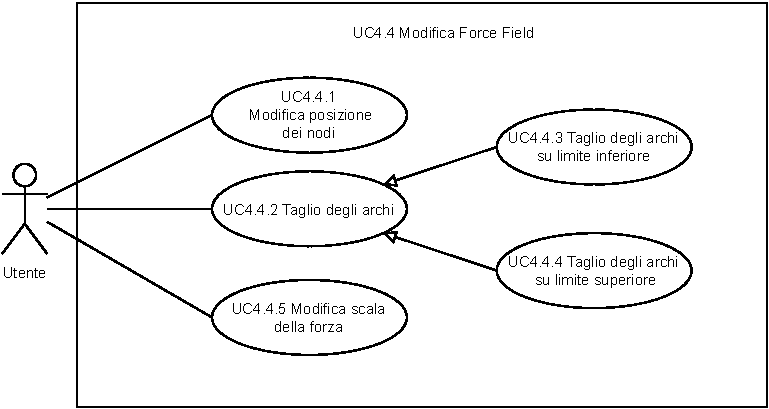
\includegraphics[width=0.6  \textwidth]{componenti/casi-duso/diagrammi/UC4_4.pdf}
    \caption{Diagramma rappresentante UC4.4}
    \label{fig:UC4.4}
\end{figure}


\begin{itemize}
    \item \textbf{Descrizione}: L’utente vuole modificare la visualizzazione del grafo Force Field
                                costruito dal dataset corrente.
	
    \item \textbf{Attore primario}: Utente.
    
    \item \textbf{Precondizione}:   La visualizzazione costruita dal dataset corrente è un Force Field.

    \item \textbf{Postcondizione}:  Viene aggiornato il grafico costruito e visualizzato con i nuovi parametri.

	\item \textbf{Scenario principale}:
		\begin{enumerate}
            \item L'utente apporta le modifiche desiderate tra quelle offerte dal Force Field.
        \end{enumerate}
\end{itemize}

\paragraph{UC4.4.1 Modifica posizione dei nodi}
\label{par:uc4.4.1}
\begin{itemize}
    \item \textbf{Descrizione}: L’utente vuole esplorare meglio i dati e decide di 
                                modificare la posizione dei nodi del grafo, trascinandoli con il 
                                cursore nell'area definita dal grafico.
	
    \item \textbf{Attore primario}: Utente.
    
    \item \textbf{Precondizione}:   La visualizzazione costruita dal dataset corrente è un Force Field.
    \item \textbf{Postcondizione}:  Viene modificata la posizione dei nodi del grafo nella visualizzazione.

	\item \textbf{Scenario principale}:
        \begin{enumerate}
            \item L'utente tiene premuto il tasto di selezione e trascina il cursore spostando il nodo nello spazio della visualizzazione.
            \item La visualizzazione muove i punti del grafo mantenendo le connessioni tra i nodi.
        \end{enumerate}
\end{itemize}

\paragraph{UC4.4.2 Taglio degli archi}
\label{par:uc4.4.2}
\begin{itemize}
    \item \textbf{Descrizione}:     L'utente imposta un valore di soglia sulla distanza, gli archi corrispondenti ad una distanza che non rispetta la soglia vengono rimossi;
    \item \textbf{Attore primario}: Utente;
    \item \textbf{Precondizione}:   La visualizzazione correntemente costruita dal dataset é un Force Field;
    \item \textbf{Postcondizione}:  Viene aggiornata la visualizzazione, rimuovendo gli archi in base al valore di soglia impostato;
    \item \textbf{Scenario principale}:
    \begin{itemize}
        \item L'utente inserisce nell'apposito campo il valore di soglia;
        \item Gli archi le cui coordinate nella matrice delle distanze non rispettano il valore di soglia vengono rimossi;
        \item La visualizzazione viene aggiornata rimuovendo gli archi secondo il valore di soglia stabilito.
    \end{itemize}
\end{itemize}

\paragraph{UC4.4.3 Taglio degli archi su limite inferiore}
\label{par:uc4.4.3}
\begin{itemize}
    \item \textbf{Descrizione}:     L'utente imposta un valore di soglia minimo sulla distanza, gli archi corrispondenti ad una distanza inferiore vengono rimossi;
    \item \textbf{Attore primario}: Utente;
    \item \textbf{Precondizione}:   La visualizzazione correntemente costruita dal dataset é un Force Field;
    \item \textbf{Postcondizione}:  Viene aggiornata la visualizzazione, rimuovendo gli archi associati ad una distanza inferiore al valore di soglia minimo;
    \item \textbf{Scenario principale}:
    \begin{itemize}
        \item L'utente inserisce nell'apposito campo il valore di soglia minimo;
        \item Gli archi le cui coordinate nella matrice delle distanze corrispondono ad una distanza inferiore al valore di soglia minimo vengono rimossi;
        \item La visualizzazione viene aggiornata rimuovendo gli archi con una distanza associata inferiore al valore di soglia minimo.
    \end{itemize}
\end{itemize}

\paragraph{UC4.4.4 Taglio degli archi su limite superiore}
\label{par:uc4.4.4}
\begin{itemize}
    \item \textbf{Descrizione}:     L'utente imposta un valore di soglia massimo sulla distanza, gli archi corrispondenti ad una distanza superiore vengono rimossi;
    \item \textbf{Attore primario}: Utente;
    \item \textbf{Precondizione}:   La visualizzazione correntemente costruita dal dataset é un Force Field;
    \item \textbf{Postcondizione}:  Viene aggiornata la visualizzazione, rimuovendo gli archi associati ad una distanza superiore al valore di soglia massimo;
    \item \textbf{Scenario principale}:
    \begin{itemize}
        \item L'utente inserisce nell'apposito campo il valore di soglia massimo;
        \item Gli archi le cui coordinate nella matrice delle distanze corrispondono ad una distanza superiore al valore di soglia massimo vengono rimossi;
        \item La visualizzazione viene aggiornata rimuovendo gli archi con una distanza associata superiore al valore di soglia massimo.
    \end{itemize}
\end{itemize}

\paragraph{UC4.4.5 Modifica scala della forza}
\label{par:uc4.4.5}
\begin{itemize}
    \item \textbf{Descrizione}: Per poter visualizzare meglio i cluster di dati l’utente 
                                decide di scalare la forza di attrattiva tra i nodi.

	
    \item \textbf{Attore primario}: Utente.
    
    \item \textbf{Precondizione}:   La visualizzazione costruita dal dataset corrente è un Force Field.
    \item \textbf{Postcondizione}:  Viene modificata l'intensità della forza attrattiva tra i nodi del grafo nella visualizzazione.

	\item \textbf{Scenario principale}:
        \begin{enumerate}
            \item L'utente seleziona la barra intensità e trascinando il cursore sulla barra varia l’intensità.
            \item La visualizzazione modifica l'intensità della forza secondo il valore selezionato nel grafo.
        \end{enumerate}
\end{itemize}

\newpage
\subsubsection{UC4.5 Modifica Distance Map}
\label{ssub:uc4.5}
% TODO: Insert image for Distance Map
\begin{figure}[h]
    \centering
    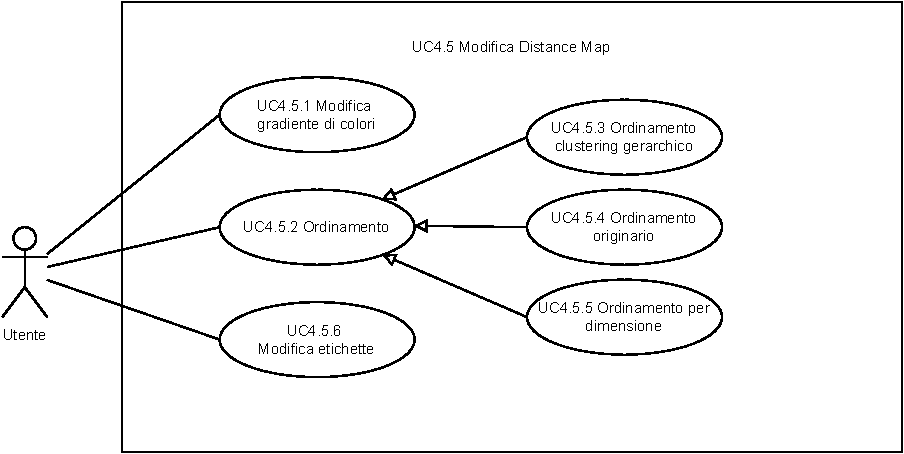
\includegraphics[width=0.8\textwidth]{componenti/casi-duso/diagrammi/UC4_5.pdf}
    \caption{Diagramma rappresentante UC4.5}
    \label{fig:UC4.5}
\end{figure}

\begin{itemize}
    \item \textbf{Descrizione}: L'utente vuole modificare la visualizzazione della Distance Map costruita dal dataset corrente;
    \item \textbf{Attore primario}: Utente;
    \item \textbf{Precondizione}: La visualizzazione costruita dal dataset corrente è un grafico di tipo Distance Map;
    \item \textbf{Postcondizione}: Viene aggiornato il grafico costruito con i nuovi parametri;
    \item \textbf{Scenario principale}: 
    \begin{itemize}
        \item L'utente apporta le modifiche desiderate tra quelle offerte dalla Distance Map.
    \end{itemize}
\end{itemize}

\paragraph{UC4.5.1 Modifica gradiente di colori}
\label{par:uc4.5.1}
\begin{itemize}
    \item \textbf{Descrizione}: L'utente vuole esplorare meglio i dati e decide di modificare la scala dei colori applicata alla Distance Map scegliendo una tra quelle proposte;
    \item \textbf{Attore primario}: Utente;
    \item \textbf{Precondizione}: La visualizzazione costruita dal dataset corrente è una Distance Map;
    \item \textbf{Postcondizione}: Viene modificata la scala dei colori del grafico nella visualizzazione.
    \item \textbf{Scenario principale}: 
    \begin{itemize}
        \item L'utente seleziona la voce "Scala dei colori" e seleziona una delle opzioni disponibili.
        \item La visualizzazione cambia la scala dei colori adottata dalla Distance Map.
    \end{itemize}
\end{itemize}

\paragraph{UC4.5.2 Ordinamento}
\label{par:uc4.5.2}
\begin{itemize}
    \item \textbf{Descrizione}: L'utente per esplorare meglio i dati decide di ordinare le righe e le colonne del Distance Map il quale aggiunge un dendrogramma alla visualizzazione corrente.
    \item \textbf{Attore primario}: Utente.
    \item \textbf{Precondizione}: La visualizzazione costruita dal dataset corrente è una Distance Map.
    \item \textbf{Postcondizione}: Le righe e le colonne del Distance Map vengono visualizzati secondo l'ordine scelto dall'utente.
    \item \textbf{Scenario principale}: 
    \begin{itemize}
        \item L'utente seleziona la casella di ordinamento.
        \item Le righe e le colonne della Distance Map vengono visualizzate secondo l'ordinamento selezionato.
    \end{itemize}
\end{itemize}

\paragraph{UC4.5.3 Ordinamento clustering gerarchico}
\label{par:uc4.5.3}
\begin{itemize}
    \item \textbf{Descrizione}: L'utente per esplorare meglio i dati decide di ordinare le righe e le colonne del Distance Map seguendo l'algoritmo di clustering gerarchico il quale aggiunge un dendrogramma alla visualizzazione corrente.
    \item \textbf{Attore primario}: Utente.
    \item \textbf{Precondizione}: La visualizzazione costruita dal dataset corrente è una Distance Map.
    \item \textbf{Postcondizione}: Le righe e le colonne del Distance Map vengono visualizzate secondo l'ordine impostato dall'algoritmo di clustering gerarchico.
    \item \textbf{Scenario principale}: 
    \begin{itemize}
        \item L'utente seleziona la casella di ordinamento delle colonne.
        \item Le righe e le colonne della Distance Map vengono visualizzate secondo l'ordinamento del clustering gerarchico, inoltre viene aggiunto il dendrogramma al grafico.
    \end{itemize}
\end{itemize}

\paragraph{UC4.5.4 Ordinamento originario}
\label{par:uc4.5.4}
\begin{itemize}
    \item \textbf{Descrizione}: L'utente per esplorare meglio i dati decide di ordinare le righe e le colonne del Distance Map seguendo l'ordine originario del dataset corrente.
    \item \textbf{Attore primario}: Utente.
    \item \textbf{Precondizione}: La visualizzazione costruita dal dataset corrente è una Distance Map.
    \item \textbf{Postcondizione}: Le righe e le colonne del Distance Map vengono visualizzate secondo l'ordine originario del dataset corrente.
    \item \textbf{Scenario principale}: 
    \begin{itemize}
        \item L'utente seleziona la casella di ordinamento delle colonne.
        \item Le righe e le colonne della Distance Map vengono visualizzate secondo l'ordine originario del dataset corrente.
    \end{itemize}
\end{itemize}

\paragraph{UC4.5.5 Ordinamento per dimensione}
\label{par:uc4.5.5}
\begin{itemize}
    \item \textbf{Descrizione}: L'utente per esplorare meglio i dati decide di ordinare le righe e le colonne del Distance Map ordinando le dimensioni per un dato algoritmo.
    \item \textbf{Attore primario}: Utente.
    \item \textbf{Precondizione}: La visualizzazione costruita dal dataset corrente è una Distance Map.
    \item \textbf{Postcondizione}: Le colonne del Distance Map vengono visualizzati secondo l'ordine impostato dall'algoritmo di ordinamento selezionato applicato alle dimensioni.
    \item \textbf{Scenario principale}: 
    \begin{itemize}
        \item L'utente seleziona la casella di ordinamento delle colonne.
        \item Le righe e le colonne della Distance Map vengono visualizzate secondo l'ordine impostato dall'algoritmo di ordinamento selezionato applicato alle dimensioni.
    \end{itemize}
\end{itemize}


\paragraph{UC4.5.6 Modifica etichette}
\label{par:uc4.5.6}
\begin{itemize}
    \item \textbf{Descrizione}: L'utente decide di modificare una o più etichette associate della Distance Map.
    \item \textbf{Attore primario}: Utente.
    \item \textbf{Precondizione}: La visualizzazione costruita dal dataset corrente è una Distance Map.
    \item \textbf{Postcondizione}: Le etichette della Distance Map vengono modificate secondo la scelta effettuata dall'utente.
    \item \textbf{Scenario principale}:
    \begin{itemize}
        \item L'utente quali etichette modificare e le modifica.
        \item Viene aggiornata la visualizzazione delle etichette nella Distance Map.
    \end{itemize}
\end{itemize}


\newpage
\subsubsection{UC4.6 Modifica Proiezione Lineare Multi Asse}
\label{ssub:uc4.6}
% TODO: Create image for PLMA
\begin{figure}[h]
    \centering
    % 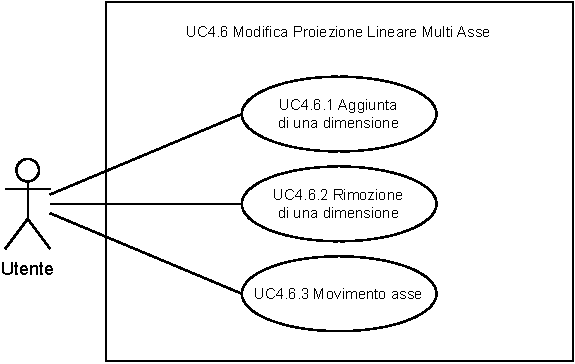
\includegraphics[width=0.8\textwidth]{componenti/casi-duso/diagrammi/UC4_6.pdf}
    \caption{Diagramma rappresentante UC4.6}
    \label{fig:UC4.6}
\end{figure}

\begin{itemize}
    \item \textbf{Descrizione}: L’utente vuole modificare la visualizzazione della Proiezione Lineare Multi Asse
                                costruita dal dataset corrente.
	
    \item \textbf{Attore primario}: Utente.
    
    \item \textbf{Precondizione}:   La visualizzazione costruita dal dataset corrente è un grafico di tipo Proiezione Lineare Multi Asse.
    \item \textbf{Postcondizione}:  Viene aggiornato il grafico costruito e visualizzato con i nuovi parametri.

	\item \textbf{Scenario principale}:
		\begin{enumerate}
            \item L'utente apporta le modifiche desiderate tra quelle offerte dalla Proiezione Lineare Multi Asse.
        \end{enumerate}
\end{itemize}

\paragraph{UC4.6.1 Aggiunta dimensione}
\label{par:uc4.6.1}
\begin{itemize}
    \item \textbf{Descrizione}: L’utente decide di visualizzare maggiori informazioni
                                aggiungendo una dimensione al grafico.

    \item \textbf{Attore primario}: Utente.
    
    \item \textbf{Precondizione}:   La visualizzazione costruita corrente è una Proiezione Lineare Multi Asse
                                    e rappresenta al più una dimensione in meno al numero di dimensioni del dataset.
    \item \textbf{Postcondizione}:  La visualizzazione della PLMA aggiunge una dimensione.

	\item \textbf{Scenario principale}:
        \begin{enumerate}
            \item L'utente seleziona la voce "Dimensioni" e seleziona una dimensione da aggiungere alla proiezione.
            \item La visualizzazione aggiunge la dimensione selezionata e riposiziona i punti.
           
        \end{enumerate}
\end{itemize}

\paragraph{UC4.6.2 Rimozione dimensione}
\label{par:uc4.6.2}
\begin{itemize}
    \item \textbf{Descrizione}: L’utente decide di rimuovere una dimensione dalla Proiezione Lineare Multi Asse
                                a patto che essa non sia monodimensionale.

    \item \textbf{Attore primario}: Utente.
    
    \item \textbf{Precondizione}:   La visualizzazione costruita dal dataset corrente è una Proiezione Lineare Multi Asse
                                    e rappresenta almeno due dimensioni.
    \item \textbf{Postcondizione}:  La visualizzazione della PLMA rimuove una dimensione.

	\item \textbf{Scenario principale}:
        \begin{enumerate}
            \item L'utente seleziona la voce "Dimensioni" e seleziona una dimensione da rimuovere dalla proiezione.
            \item La visualizzazione rimuove la dimensione selezionata e riposiziona i punti.
           
        \end{enumerate}
\end{itemize}

\paragraph{UC4.6.3 Rotazione asse}
\label{par:uc4.6.3}
\begin{itemize}
    \item \textbf{Descrizione}: L'utente decide di spostare gli assi per poter visualizzare diverse proiezioni dello stesso dataset.
    \item \textbf{Attore primario}: Utente.
    \item \textbf{Precondizione}: La visualizzazione costruita dal dataset corrente è una Proiezione Lineare Multi Asse.
    \item \textbf{Postcondizione}: Il grafico viene ridisegnato con gli assi opportunamente ri-orientati.
    \item \textbf{Scenario principale}:
    \begin{enumerate}
        \item L'utente cliccando con il mouse su un asse del grafico trascina l'asse ri-orientandolo.
	\item La visualizzazione viene aggiornata con l'asse ri-orientato.
    \end{enumerate}
\end{itemize}

\newpage
\subsubsection{UC4.7 Modifica Heat Map}
\label{ssub:uc4.7}
% TODO: Create image for force field graph.
\begin{figure}[h]
    \centering
    % 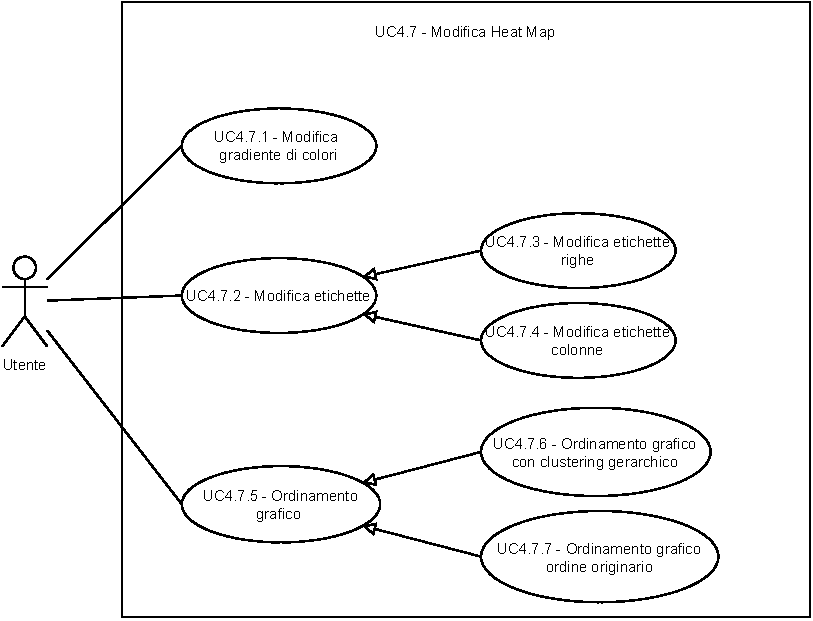
\includegraphics[width=0.6\textwidth]{componenti/casi-duso/diagrammi/UC4_7.pdf}
    \caption{Diagramma rappresentante UC4.7}
    \label{fig:UC4.7}
\end{figure}


\begin{itemize}
    \item \textbf{Descrizione}: L’utente modifica la visualizzazione della Heat Map correntemente visualizzata;
	
    \item \textbf{Attore primario}: Utente;
    
    \item \textbf{Precondizione}:   La visualizzazione correntemente costruita dal dataset è una Heat Map;

    \item \textbf{Postcondizione}:  Viene aggiornata la visualizzazione secondo i nuovi parametri impostati;

	\item \textbf{Scenario principale}:
		\begin{enumerate}
            \item L'utente apporta le modifiche desiderate tra quelle offerte dalla Heat Map.
        \end{enumerate}
\end{itemize}

\paragraph{UC4.7.1 Modifica gradiente di colori}
\label{par:uc4.7.1}
\begin{itemize}
    \item \textbf{Descrizione}: L’utente modifica il gradiente di colori applicato alla Heat Map scegliendone uno tra quelli proposti;
	
    \item \textbf{Attore primario}: Utente;
    
    \item \textbf{Precondizione}:   La visualizzazione correntemente costruita dal dataset è una Heat Map;
    \item \textbf{Postcondizione}:  Il gradiente di colori utilizzato nella visualizzazione della Heat Map é quello selezionato dall'utente;

	\item \textbf{Scenario principale}:
        \begin{enumerate}
            \item L'utente seleziona la voce "Colori" e seleziona una delle opzioni disponibili;
            \item La visualizzazione modifica il gradiente di colori utilizzato, impostando quello selezionato dall'utente;
            \item La visualizzazione viene aggiornata secondo il gradiente di colori impostato.
        \end{enumerate}
\end{itemize}

\paragraph{UC4.7.2 Modifica asse}
\label{par:uc4.7.2}
\begin{itemize}
    \item \textbf{Descrizione}:     L'utente modifica le proprietà dell'asse dell'Heat Map correntemente visualizzata;
    \item \textbf{Attore primario}: Utente;

    \item \textbf{Precondizione}:   La visualizzazione correntemente costruita dal dataset é una Heat Map;
    \item \textbf{Postcondizione}:  Le proprietà visive dell'asse vengono modificate secondo quanto selezionato;
    \item \textbf{Scenario principale}:
    \begin{enumerate}
        \item L'utente mediante l'apposito bottone effettua l'ordinamento dell'asse della visualizzazione (\hyperref[spar:uc4.7.2.2]{UC4.7.2.2});
    \end{enumerate}
    \item \textbf{Scenario secondario}:
    \begin{enumerate}
        \item L'utente mediante l'apposito bottone modifica la categoria di etichette associata all'asse della visualizzazione (\hyperref[spar:uc4.7.2.1]{UC4.7.2.1});
    \end{enumerate}
    \item \textbf{Generalizzazioni}: 
    \begin{itemize}
        \item Modifica righe (\hyperref[par:uc4.7.3]{UC4.7.3});
        \item Modifica colonne (\hyperref[par:uc4.7.4]{UC4.7.4}).
    \end{itemize}
\end{itemize}

\subparagraph{UC4.7.2.1 Modifica etichette}
\label{spar:uc4.7.2.1}
\begin{itemize}
    \item \textbf{Descrizione}:     L'utente modifica la categoria di etichette associata all'asse della visualizzazione;
    \item \textbf{Attore primario}: Utente;
    \item \textbf{Precondizione}:   La visualizzazione correntemente costruita dal dataset é una Heat Map ed é stato selezionato il bottone "Etichette" all'interno del campo "Asse";
    \item \textbf{Postcondizione}:  La categoria di etichette dell'asse della visualizzazione viene modificata;
    \item \textbf{Scenario principale}:
    \begin{enumerate}
        \item L'utente seleziona una tra le possibili categorie di etichette applicabili, mostrategli in seguito alla pressione del bottone "Etichette";
        \item La categoria di etichette dell'asse viene modificata in base a quanto precedentemente selezionato.
    \end{enumerate}
\end{itemize}

\subparagraph{UC4.7.2.2 Ordinamento}
\label{spar:uc4.7.2.2}
\begin{itemize}
    \item \textbf{Descrizione}:     L'utente modifica l'ordinamento degli elementi dell'asse della visualizzazione;
    \item \textbf{Attore primario}: Utente;
    \item \textbf{Precondizione}:   La visualizzazione correntemente costruita dal dataset é una Heat Map ed é stato selezionato il bottone "Ordina";
    \item \textbf{Postcondizione}:  L'ordine degli elementi dell'asse viene modificato;
    \item \textbf{Scenario principale}:
    \begin{enumerate}
        \item L'utente seleziona uno tra i possibili ordinamenti degli elementi dell'asse, mostratigli in seguito alla pressione del bottone "Ordina" all'interno del campo "Asse";
        \item L'ordinamento degli elementi dell'asse della visualizzazione viene modificato in base a quanto precedentemente selezionato.
    \end{enumerate}
    \item \textbf{Generalizzazioni}:
    % \begin{itemize}
    %     \item Ordinamento clustering gerarchico (\hyperref[spar:uc4.7.2.3]{UC4.7.2.3})
    %     \item Ordinamento originario (\hyperref[spar:uc4.7.2.4{UC4.7.2.4})
    % \end{itemize}
\end{itemize}

\subparagraph{UC4.7.2.3 Ordinamento clustering gerarchico}
\label{spar:uc4.7.2.3}
\begin{itemize}
    \item \textbf{Descrizione}:     L'utente modifica l'ordinamento degli elementi dell'asse della visualizzazione con il clustering gerarchico;
    \item \textbf{Attore primario}: Utente;
    \item \textbf{Precondizione}:   La visualizzazione correntemente costruita dal dataset é una Heat Map ed é stato selezionato il bottone "Ordina" all'interno del campo "Asse";
    \item \textbf{Postcondizione}:  L'ordine degli elementi dell'asse viene modificato in accordo con il risultato dell'applicazione dell'algoritmo di clustering gerarchico;
    \item \textbf{Scenario principale}:
    \begin{enumerate}
        \item L'utente seleziona l'ordinamento degli elementi con clustering gerarchico;
        \item L'ordinamento degli elementi dell'asse della visualizzazione viene modificato in base al risultato dell'algoritmo di clustering gerarchico;
        \item Viene aggiunto sull'asse di visualizzazione il dendrogramma associato alla clusterizzazione.
    \end{enumerate}
\end{itemize}

\subparagraph{UC4.7.2.4 Ordinamento originale}
\label{spar:uc4.7.2.4}
\begin{itemize}
    \item \textbf{Descrizione}:     L'utente modifica l'ordinamento degli elementi dell'asse della visualizzazione all'ordine originale dei dati;
    \item \textbf{Attore primario}: Utente;
    \item \textbf{Precondizione}:   La visualizzazione correntemente costruita dal dataset é una Heat Map ed é stato selezionato il bottone "Ordina" all'interno del campo "Asse";
    \item \textbf{Postcondizione}:  L'ordine degli elementi dell'asse viene modificato in accordo con l'ordine originale dei dati;
    \item \textbf{Scenario principale}:
    \begin{enumerate}
        \item L'utente seleziona l'ordinamento degli elementi originale;
        \item L'ordinamento degli elementi dell'asse della visualizzazione viene modificato in base all'ordine originale dei dati.
    \end{enumerate}
\end{itemize}

\paragraph{UC4.7.3 Modifica righe}
\label{par:uc4.7.3}
\begin{itemize}
    \item \textbf{Descrizione}:     L'utente modifica le proprietà delle righe dell'Heat Map correntemente visualizzata;
    \item \textbf{Attore primario}: Utente;
    \item \textbf{Precondizione}:   La visualizzazione correntemente costruita dal dataset é una Heat Map;
    \item \textbf{Postcondizione}:  Le proprietà visive delle righe vengono modificate secondo quanto selezionato;
    
    \item \textbf{Scenario principale}:
    \begin{enumerate}
        \item L'utente mediante l'apposito bottone effettua l'ordinamento delle righe della visualizzazione (\hyperref[spar:uc4.7.3.2]{UC4.7.3.2});
    \end{enumerate}
    \item \textbf{Scenario secondario}:
    \begin{enumerate}
        \item L'utente mediante l'apposito bottone modifica la categoria di etichette associata alle righe della visualizzazione (\hyperref[spar:uc4.7.3.1]{UC4.7.3.1}).
    \end{enumerate}
\end{itemize}
    
\subparagraph{UC4.7.3.1 Modifica etichette righe}
\label{spar:uc4.7.3.1}
\begin{itemize}
    \item \textbf{Descrizione}:     L'utente modifica la categoria di etichette associata alle righe della visualizzazione;
    \item \textbf{Attore primario}: Utente;
    \item \textbf{Precondizione}:   La visualizzazione correntemente costruita dal dataset é una Heat Map ed é stato selezionato il bottone "Etichette" all'interno del campo "Righe";
    \item \textbf{Postcondizione}:  La categoria di etichette delle righe della visualizzazione viene modificata;
    \item \textbf{Scenario principale}:
    \begin{enumerate}
        \item L'utente seleziona una tra le possibili categorie di etichette applicabili, mostrategli in seguito alla pressione del bottone "Etichette";
        \item La categoria di etichette delle righe viene modificata in base a quanto precedentemente selezionato.
    \end{enumerate}
\end{itemize}

\subparagraph{UC4.7.3.2 Ordinamento righe}
\label{spar:uc4.7.3.2}
\begin{itemize}
    \item \textbf{Descrizione}:     L'utente modifica l'ordinamento delle righe della visualizzazione;
    \item \textbf{Attore primario}: Utente;
    \item \textbf{Precondizione}:   La visualizzazione correntemente costruita dal dataset é una Heat Map ed é stato selezionato il bottone "Ordina" all'interno del campo "Righe";
    \item \textbf{Postcondizione}:  L'ordine delle righe viene modificato;
    \item \textbf{Scenario principale}:
    \begin{enumerate}
        \item L'utente seleziona uno tra i possibili ordinamenti delle righe, mostratigli in seguito alla pressione del bottone "Ordina";
        \item L'ordinamento delle righe della visualizzazione viene modificato in base a quanto precedentemente selezionato.
    \end{enumerate}
    \item \textbf{Generalizzazioni}:
    % \begin{itemize}
    %     \item Ordinamento clustering gerarchico (\hyperref[spar:uc4.7.3.3]{UC4.7.3.3})
    %     \item Ordinamento originario (\hyperref[spar:uc4.7.3.4{UC4.7.3.4})
    % \end{itemize}
\end{itemize}

\subparagraph{UC4.7.3.3 Ordinamento righe clustering gerarchico}
\label{spar:uc4.7.3.3}
\begin{itemize}
    \item \textbf{Descrizione}:     L'utente modifica l'ordinamento delle righe della visualizzazione con il clustering gerarchico;
    \item \textbf{Attore primario}: Utente;
    \item \textbf{Precondizione}:   La visualizzazione correntemente costruita dal dataset é una Heat Map ed é stato selezionato il bottone "Ordina" all'interno del campo "Righe";
    \item \textbf{Postcondizione}:  L'ordine delle righe viene modificato in accordo con il risultato dell'applicazione dell'algoritmo di clustering gerarchico;
    \item \textbf{Scenario principale}:
    \begin{enumerate}
        \item L'utente seleziona l'ordinamento delle righe con clustering gerarchico;
        \item L'ordinamento delle righe della visualizzazione viene modificato in base al risultato dell'algoritmo di clustering gerarchico;
        \item Viene aggiunto sull'asse verticale il dendrogramma associato alla clusterizzazione.
    \end{enumerate}
\end{itemize}

\subparagraph{UC4.7.3.4 Ordinamento righe originale}
\label{spar:uc4.7.3.4}
\begin{itemize}
    \item \textbf{Descrizione}:     L'utente modifica l'ordinamento delle righe della visualizzazione all'ordine originale dei dati;
    \item \textbf{Attore primario}: Utente;
    \item \textbf{Precondizione}:   La visualizzazione correntemente costruita dal dataset é una Heat Map ed é stato selezionato il bottone "Ordina" all'interno del campo "Righe";
    \item \textbf{Postcondizione}:  L'ordine delle righe viene modificato in accordo con l'ordine originale dei dati;
    \item \textbf{Scenario principale}:
    \begin{enumerate}
        \item L'utente seleziona l'ordinamento delle righe originale;
        \item L'ordinamento delle righe viene modificato in base all'ordine originale dei dati.
    \end{enumerate}
\end{itemize}

\subparagraph{UC4.7.3.5 Ordinamento righe con dimensione}
\label{spar:uc4.7.3.5}
\begin{itemize}
    \item \textbf{Descrizione}:     L'utente modifica l'ordinamento delle righe della visualizzazione secondo i valori di una dimensione selezionata;
    \item \textbf{Attore primario}: Utente;
    \item \textbf{Precondizione}:   La visualizzazione correntemente costruita dal dataset é una Heat Map ed é stato selezionato il bottone "Ordina" all'interno del campo "Righe";
    \item \textbf{Postcondizione}:  L'ordine delle righe viene modificato in accordo con l'ordine della dimensione selezionata;
    \item \textbf{Scenario principale}:
    \begin{enumerate}
        \item L'utente seleziona l'ordinamento secondo dimensione;
        \item L'utente seleziona secondo quale dimensione desidera ordinare le righe;
        \item L'ordinamento delle righe viene modificato in base all'ordine della dimensione scelta.
    \end{enumerate}
\end{itemize}

\paragraph{UC4.7.4 Modifica colonne}
\label{par:uc4.7.4}
\begin{itemize}
    \item \textbf{Descrizione}:     L'utente modifica le proprietà delle colonne dell'Heat Map correntemente visualizzata;
    \item \textbf{Attore primario}: Utente;
    \item \textbf{Precondizione}:   La visualizzazione correntemente costruita dal dataset é una Heat Map;
    \item \textbf{Postcondizione}:  Le proprietà visive delle colonne vengono modificate secondo quanto selezionato;
    
    \item \textbf{Scenario principale}:
    \begin{enumerate}
        \item L'utente mediante l'apposito bottone effettua l'ordinamento delle colonne della visualizzazione (\hyperref[spar:uc4.7.4.2]{UC4.7.4.2});
    \end{enumerate}
    \item \textbf{Scenario secondario}:
    \begin{enumerate}
        \item L'utente mediante l'apposito bottone modifica la categoria di etichette associata alle colonne della visualizzazione (\hyperref[spar:uc4.7.4.1]{UC4.7.4.1}).
    \end{enumerate}
\end{itemize}

\subparagraph{UC4.7.4.1 Modifica etichette colonne}
\label{spar:uc4.7.4.1}
\begin{itemize}
    \item \textbf{Descrizione}:     L'utente modifica la categoria di etichette associata alle colonne della visualizzazione;
    \item \textbf{Attore primario}: Utente;
    \item \textbf{Precondizione}:   La visualizzazione correntemente costruita dal dataset é una Heat Map ed é stato selezionato il bottone "Etichette" all'interno del campo "Colonne";
    \item \textbf{Postcondizione}:  La categoria di etichette delle colonne della visualizzazione viene modificata;
    \item \textbf{Scenario principale}:
    \begin{enumerate}
        \item L'utente seleziona una tra le possibili categorie di etichette applicabili, mostrategli in seguito alla pressione del bottone "Etichette";
        \item La categoria di etichette delle colonne viene modificata in base a quanto precedentemente selezionato.
    \end{enumerate}
\end{itemize}

\subparagraph{UC4.7.4.2 Ordinamento colonne}
\label{spar:uc4.7.4.2}
\begin{itemize}
    \item \textbf{Descrizione}:     L'utente modifica l'ordinamento delle colonne della visualizzazione;
    \item \textbf{Attore primario}: Utente;
    \item \textbf{Precondizione}:   La visualizzazione correntemente costruita dal dataset é una Heat Map ed é stato selezionato il bottone "Ordina" all'interno del campo "Colonne";
    \item \textbf{Postcondizione}:  L'ordine delle colonne viene modificato;
    \item \textbf{Scenario principale}:
    \begin{enumerate}
        \item L'utente seleziona uno tra i possibili ordinamenti delle colonne, mostratigli in seguito alla pressione del bottone "Ordina";
        \item L'ordinamento delle colonne della visualizzazione viene modificato in base a quanto precedentemente selezionato.
    \end{enumerate}
    \item \textbf{Generalizzazioni}:
    % \begin{itemize}
    %     \item Ordinamento clustering gerarchico (\hyperref[spar:uc4.7.4.3]{UC4.7.4.3})
    %     \item Ordinamento originario (\hyperref[spar:uc4.7.4.4{UC4.7.4.4})
    % \end{itemize}
\end{itemize}

\subparagraph{UC4.7.4.3 Ordinamento colonne clustering gerarchico}
\label{spar:uc4.7.4.3}
\begin{itemize}
    \item \textbf{Descrizione}:     L'utente modifica l'ordinamento delle colonne della visualizzazione con il clustering gerarchico;
    \item \textbf{Attore primario}: Utente;
    \item \textbf{Precondizione}:   La visualizzazione correntemente costruita dal dataset é una Heat Map ed é stato selezionato il bottone "Ordina" all'interno del campo "Colonne";
    \item \textbf{Postcondizione}:  L'ordine delle colonne viene modificato in accordo con il risultato dell'applicazione dell'algoritmo di clustering gerarchico;
    \item \textbf{Scenario principale}:
    \begin{enumerate}
        \item L'utente seleziona l'ordinamento delle colonne con clustering gerarchico;
        \item L'ordinamento delle colonne della visualizzazione viene modificato in base al risultato dell'algoritmo di clustering gerarchico;
        \item Viene aggiunto sull'asse orizzontale il dendrogramma associato alla clusterizzazione.
    \end{enumerate}
\end{itemize}

\subparagraph{UC4.7.4.4 Ordinamento colonne originale}
\label{spar:uc4.7.4.4}
\begin{itemize}
    \item \textbf{Descrizione}:     L'utente modifica l'ordinamento delle colonne della visualizzazione all'ordine originale delle dimensioni;
    \item \textbf{Attore primario}: Utente;
    \item \textbf{Precondizione}:   La visualizzazione correntemente costruita dal dataset é una Heat Map ed é stato selezionato il bottone "Ordina" all'interno del campo "Colonne";
    \item \textbf{Postcondizione}:  L'ordine delle colonne viene modificato in accordo con l'ordine originale delle dimensioni;
    \item \textbf{Scenario principale}:
    \begin{enumerate}
        \item L'utente seleziona l'ordinamento delle colonne originale;
        \item L'ordinamento delle colonne viene modificato in base all'ordine originale delle dimensioni.
    \end{enumerate}
\end{itemize}

\paragraph{UC4.7.5 Modifica dimensione}
\label{par:uc4.7.5}
\begin{itemize}
    \item \textbf{Descrizione}:     L'utente modifica le dimensioni visualizzate nella visualizzazione;
    \item \textbf{Attore primario}: Utente;

    \item \textbf{Precondizione}:   La visualizzazione correntemente costruita dal dataset é una Heat Map;
    \item \textbf{Postcondizione}:  La visualizzazione viene aggiornata in accordo con le modifiche di rappresentazione delle dimensioni effettuate;
    \item \textbf{Scenario principale}:
    \begin{enumerate}
        \item L'utente seleziona il pulsante "Rimuovi" in una tra le dimensioni correntemente visualizzate;
        \item La dimensione selezionata viene rimossa dalla visualizzazione;
        \item La visualizzazione viene aggiornata in accordo con le modifiche di rappresentazione  delle dimensioni effettuate;
    \end{enumerate}
    \item \textbf{Scenario alternativo}: 
    \begin{enumerate}
        \item L'utente seleziona il pulsante "Aggiungi" in una tra le dimensioni correntemente non visualizzate;
        \item La dimensione selezionata viene aggiunta alla visualizzazione;
        \item La visualizzazione viene aggiornata in accordo con le modifiche di rappresentazione  delle dimensioni effettuate.
    \end{enumerate}
\end{itemize}

\subsection{UC4.8 Annullamento delle modifiche}
\label{ssub:uc4.8}
\begin{itemize}
    \item \textbf{Descrizione}: L'utente decide di scartare le modifiche fatte nella corrente selezione di modifica.

    \item \textbf{Attore primario}: Utente.
    
    \item \textbf{Precondizione}:   L'utente ha selezionato la voce di Modifica Grafico dal menu.
    \item \textbf{Postcondizione}:  Viene ripristinato il grafo ai parametri precedenti della selezione e visualizzato.

	\item \textbf{Scenario principale}:
        \begin{enumerate}

            \item L'utente seleziona il pulsante "Annulla modifiche".
            \item HD Viz ripristina i parametri del grafo ai valori precedenti alla selezione del menu di modifica.
        
        \end{enumerate}
\end{itemize}



